% report.tex

\documentclass[a4paper,11pt]{article}

% Import packages
\usepackage[a4paper]{geometry}
\usepackage[utf8]{inputenc}
\usepackage{amsmath}
\usepackage{amssymb}
\usepackage{graphicx}


% Change enumerate environments you use letters
\renewcommand{\theenumi}{\alph{enumi}}

% Set title, author name and date
\title{Chitty-Chat}
\author{Johannes Jørgensen,} 
\date{\today}

\begin{document} 

\maketitle

\subsection*{Streaming in Chitty-Chat}
This version of Chitty-Chat is implemented using bidirectional streaming. Which allows for messages to be sent over a single stream.
Every message include the author who send said message. When a message goes from the client only the id is sent, but is changed to the name when the server broadcasts.

Chitty-Chat could also be implemented using server-side streaming with an publish endpoint.
A client could then subscribe to the message stream, where the server will send (broadcast) the published messages.
Another service endpoint would then be used to publish the messages.
This would also allow for different Author signup and TextMessage types in the proto file, where the first text message currently is handled as is if it were an author.

\subsection*{Describe your system architecture - do you have a server-client architecture, peer-to-peer, or something else?}
\subsection*{Describe what  RPC methods are implemented, of what type, and what messages types are used for communication}
We have implemented a single RPC method called \verb|JoinConversation| that both takes and return a \textit{stream} of type \verb|Message|.
The \verb|Message| type is the message type used for communication. It contains the fields:
\begin{itemize}
    \item \verb|timestamp|: A Lamport timestamp
    \item \verb|username|: The username of the sender
    \item \verb|content|: The content of the message
\end{itemize} 

\subsection*{Describe how you have implemented the calculation of the Lamport timestamps}

Both the server and the client have a \verb|Lamport| clock initilized on start, that is set to \verb|0|. This is also the case for newcomers that connect to the server. 
The \verb|Lamport| clock is handled with these conditions:\\
\textbf{Client:}
\begin{itemize}
    \item When a client sends a message, the \verb|Lamport| clock is incremented by \verb|1|.
    \item When a client receives a message, the \verb|Lamport| clock is incremented by \verb|1| if the timestamp of the received message is greater than the current \verb|Lamport| clock.
\end{itemize}
\textbf{Server:}
\begin{itemize}
    \item When the server receives a message, the \verb|Lamport| clock is incremented by \verb|1| if the timestamp of the received message is greater than the current \verb|Lamport| clock.
    \item When the server broadcasts a message, the \verb|Lamport| will be incremented by \verb|1|.
    \item If a client disconnectes from the server, \verb|Lamport| clock is incremented by \verb|1| - Then the server will broadcast the disconnection.
    \item If a client connects to the server, \verb|Lamport| clock is incremented by \verb|1|- Then the server will broadcast the disconnection.
\end{itemize}
\subsection*{Provide a diagram, that traces a sequence of RPC calls together with the Lamport timestamps}
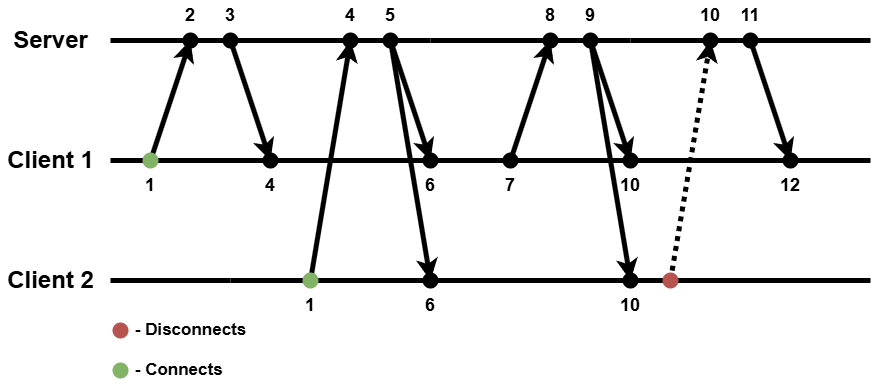
\includegraphics[width=\textwidth]{chat.png}

\subsection*{Provide a diagram, that traces a sequence of RPC calls together with the Lamport timestamps, that corresponds to a chosen sequence of interactions: Client X joins, Client X Publishes, ..., Client X leaves. Include documentation (system logs) in your appendix.}

\subsection*{Git}
[GitHub](https://github.com/ITU-DISYS2024-CENTRALIZEDSYSTEMS/Chitty-Chat)

\subsection*{Appendix}


\end{document}